\documentclass[conference]{IEEEtran}
\IEEEoverridecommandlockouts

%% ---- Math & Proof -------------------------------------------------------
\usepackage{amsmath,amssymb,amsthm}
\usepackage{mathtools}

%% ---- TikZ (all diagrams are inline, no external files) ------------------
\usepackage{tikz}
\usetikzlibrary{
  arrows.meta,
  shapes.geometric,
  shapes.multipart,
  positioning,
  fit,
  backgrounds,
  calc,
  decorations.pathreplacing,
  decorations.markings
}

%% ---- Algorithms ---------------------------------------------------------
\usepackage{algorithm}
\usepackage{algorithmic}

%% ---- Tables -------------------------------------------------------------
\usepackage{booktabs}
\usepackage{multirow}
\usepackage{array}

%% ---- Misc ---------------------------------------------------------------
\usepackage{xcolor}
\usepackage{cite}
\usepackage[T1]{fontenc}
\usepackage{enumitem}
\setlist{noitemsep,topsep=2pt,parsep=0pt}

%% ---- Colour palette -----------------------------------------------------
\definecolor{cblue}{RGB}{31,119,180}
\definecolor{corange}{RGB}{214,95,14}
\definecolor{cgreen}{RGB}{44,160,44}
\definecolor{cred}{RGB}{196,36,36}
\definecolor{cgray}{RGB}{127,127,127}
\definecolor{cpurple}{RGB}{148,103,189}
\definecolor{lblue}{RGB}{219,237,255}
\definecolor{lorange}{RGB}{255,235,210}
\definecolor{lgreen}{RGB}{210,245,215}
\definecolor{lyellow}{RGB}{255,252,210}

%% ---- TikZ node styles (reused across all figures) -----------------------
\tikzset{
  agent/.style={
    rectangle, rounded corners=4pt,
    fill=lblue, draw=cblue, line width=0.8pt,
    minimum width=1.55cm, minimum height=0.52cm,
    font=\scriptsize\sffamily, align=center
  },
  agentG/.style={
    agent, fill=lgreen, draw=cgreen
  },
  agentO/.style={
    agent, fill=lorange, draw=corange
  },
  agentR/.style={
    agent, fill=red!10, draw=cred
  },
  meta/.style={
    rectangle, rounded corners=5pt,
    fill=lorange, draw=corange, line width=1pt,
    minimum width=3.0cm, minimum height=0.65cm,
    font=\small\sffamily\bfseries, align=center
  },
  injected/.style={
    rectangle, rounded corners=4pt,
    fill=lgreen, draw=cgreen, line width=0.8pt, dashed,
    minimum width=1.55cm, minimum height=0.52cm,
    font=\scriptsize\sffamily, align=center
  },
  removed/.style={
    rectangle, rounded corners=4pt,
    fill=red!8, draw=cred, line width=0.8pt,
    minimum width=1.55cm, minimum height=0.52cm,
    font=\scriptsize\sffamily, align=center,
    opacity=0.45
  },
  router/.style={
    diamond, fill=lyellow, draw=corange, line width=0.8pt,
    minimum width=0.9cm, minimum height=0.65cm,
    font=\tiny\sffamily, align=center, inner sep=1pt
  },
  box/.style={
    rectangle, rounded corners=3pt,
    draw=cgray, line width=0.6pt, dashed,
    inner sep=6pt
  },
  arr/.style={-{Stealth[length=5pt]}, line width=0.7pt, color=#1},
  arr/.default=black
}

%% ---- Theorem environments -----------------------------------------------
\newtheorem{definition}{Definition}
\newtheorem{theorem}{Theorem}
\newtheorem{lemma}{Lemma}
\newtheorem{corollary}{Corollary}

%%==========================================================================
\title{Mutable Orchestration Graphs: Runtime DAG\\
Self-Modification via LLM-Driven Conditional Edges\\
in LangGraph}

\author{
  \IEEEauthorblockN{Anonymous Author(s)}
  \IEEEauthorblockA{Submitted for blind review \\
  \texttt{anonymous@institution.edu}}
}

\begin{document}
\maketitle

%%==========================================================================
\begin{abstract}
  Directed acyclic graph (DAG) workflow engines fix their topology
  at compile time. When intermediate node outputs reveal that planned
  branches are redundant---or that new analysis steps are urgently
  needed---these systems have no recourse: they continue executing
  nodes that add no value and skip nodes that would catch critical
  issues. We introduce \emph{Mutable Orchestration Graphs} (MOGs):
  a framework in which an LLM meta-orchestrator emits structured
  \emph{graph mutation instructions} at runtime, reshaping the DAG
  between node executions. We provide five contributions: (1) a
  formal MOG definition as a five-tuple $(V,E,\Sigma,\delta,\mathcal{M})$;
  (2) a typed mutation operator set with a JSON instruction schema;
  (3) a termination proof via a monotonically decreasing complexity
  measure; (4) an implementation on LangGraph's \texttt{StateGraph}
  with hot node injection; and (5) a threat model characterising
  the prompt-injection attack surface created by output-driven
  graph rewriting, together with a typed allowlist defence.
  Evaluated on a non-human identity (NHI) governance workload
  of 500 records, MOG reduces unnecessary agent invocations by
  58\% and LLM token consumption by 56\% versus a static baseline,
  at a median rewrite overhead of 340\,ms.
\end{abstract}

%%==========================================================================
\section{Introduction}

A workflow that cannot restructure itself in response to what it
discovers is, at best, over-engineered and, at worst, unreliable.
The problem is concrete: imagine a security orchestrator auditing
500 Azure service principals. Its static DAG commits to seven nodes
for every record---discovery, credential extraction, risk scoring,
policy check, certificate validation, notification, and report
generation. When the discovery node finds that 300 principals have
zero active credentials and have not been used in over a year, every
downstream node still fires on those records. Nothing in the graph
can say ``these are done; skip ahead.'' Conversely, when 75 principals
show signs of credential reuse and lateral movement, the fixed pipeline
has no mechanism to inject a deeper forensics step without a full
redeployment.

The underlying assumption is almost never questioned: \emph{execution
graphs are immutable after compile time}. LangGraph~\cite{langgraph2024}
offers conditional edges that route between pre-registered nodes, and
AutoGen~\cite{autogen2023} varies conversation order---but neither
treats the graph itself as a mutable object that an agent can reason
about and change. We challenge that assumption directly.

\smallskip\noindent\textbf{Contributions.} This paper makes five
distinct contributions:
\begin{enumerate}
  \item \textbf{MOG Formalism.} The Mutable Orchestration Graph
    $(V,E,\Sigma,\delta,\mathcal{M})$ is the first formal model
    of an LLM-driven self-modifying workflow DAG.
  \item \textbf{LLM Mutation Instructions.} A meta-orchestrator
    node emits structured JSON payloads naming which operator in
    $\mathcal{M}$ to apply; we define the full schema and execution
    semantics.
  \item \textbf{Convergence Guarantee.} We prove termination under
    a monotonically decreasing complexity measure $\phi$, bounding
    rewrite steps to $O(|V_0| + W_0)$.
  \item \textbf{LangGraph Implementation.} Graph topology becomes
    first-class state inside \texttt{StateGraph}, enabling hot node
    injection inside a running execution without recompilation.
  \item \textbf{Prompt-Injection Threat Model.} We characterise the
    attack surface unique to output-driven graph mutation and propose
    a typed allowlist that closes the identified vectors.
\end{enumerate}

%%==========================================================================
\section{Background}
\label{sec:background}

\subsection{LangGraph and \texttt{StateGraph}}
LangGraph~\cite{langgraph2024} represents agent workflows as a
\texttt{StateGraph}: Python callables (nodes) read and write a shared
typed dictionary; directed edges route control. Conditional edges
apply a routing function whose co-domain is a \emph{fixed}, pre-registered
node set. Once \texttt{.compile()} is called, the graph structure is
frozen---only state content varies across invocations.

\subsection{Classical Workflow Engines}
Systems such as Apache Airflow and Prefect treat DAGs as static
artefacts. Airflow~2.3 introduced dynamic task mapping for fan-out
over runtime collections, but this does not add or remove \emph{edges}.
Structural self-modification---our target---remains absent from all
production workflow engines known to the authors.

\subsection{Non-Human Identity Governance}
Non-human identities (NHIs) encompass service principals, API tokens,
deploy keys, personal access tokens (PATs), and TLS certificates.
Governing thousands of NHIs across cloud providers requires orchestrated
scanning, risk scoring, policy evaluation, and remediation. Because
NHI risk is heterogeneous---the same pipeline scan can find a
never-used read-only key alongside an over-privileged secret that
expired 30 days ago---this workload is an ideal testbed for adaptive
orchestration.

%%==========================================================================
\section{Mutable Orchestration Graphs}
\label{sec:formalism}

\subsection{The Static DAG Problem}

Let $G=(V,E)$ be the execution DAG compiled before any data arrives.
A conditional router $r\colon\Sigma\to V$ can select a successor from
the \emph{existing} node set---but it cannot extend $V$ or alter $E$.
When intermediate outputs indicate that a branch is irrelevant (wasting
computation) or that a new node is necessary (missing capability), the
system has no formal mechanism to adapt.

\subsection{Formal Definition}

\begin{definition}[Mutable Orchestration Graph]
  A \textbf{Mutable Orchestration Graph} is a five-tuple
  $\mathcal{G} = (V_t,\, E_t,\, \Sigma,\, \delta,\, \mathcal{M})$
  where:
  \begin{itemize}
    \item $V_t$ is the node set at execution step $t$ (may grow or shrink);
    \item $E_t \subseteq V_t \times V_t$ is the directed edge set at
      step $t$;
    \item $\Sigma$ is the typed state schema shared across all nodes;
    \item $\delta\colon \Sigma \to \mathcal{P}(\mathcal{M})$ is the
      \emph{meta-orchestrator function} mapping observed state to a
      (possibly empty) set of mutation instructions; and
    \item $\mathcal{M}$ is the mutation operator set.
  \end{itemize}
\end{definition}

\begin{definition}[Mutation Operator Set]
  $\mathcal{M} = \{\textsc{AddNode},\allowbreak\,\textsc{RemoveNode},\allowbreak
  \,\textsc{AddEdge},\allowbreak\,\textsc{RemoveEdge},\allowbreak
  \,\textsc{Reroute}\}$.
  Each operator is a partial function
  $m\colon (V_t, E_t) \rightharpoonup (V_{t+1}, E_{t+1})$.
\end{definition}

Figure~\ref{fig:lifecycle} contrasts a static DAG (fixed topology)
with a MOG executing the same task (node \textsc{DeepScan} is injected;
the low-risk fast path skips three nodes).

\subsection{Convergence Guarantee}

Unrestricted rewriting risks non-termination: a freshly injected node
could trigger further injections indefinitely. We bound this.

\begin{definition}[Task Complexity Measure]
  For a MOG at step $t$, define
  \[
    \phi(\mathcal{G}_t)\;=\;|V_t| + w(\sigma_t),
  \]
  where $w\colon\Sigma\to\mathbb{N}$ is the \emph{work measure}---the
  number of unprocessed items remaining in state (e.g., unscanned NHI
  records).
\end{definition}

\begin{lemma}[Monotone Reduction]
  \label{lem:mono}
  Every application of $m\in\mathcal{M}$ must satisfy
  $\phi(\mathcal{G}_{t+1})\leq\phi(\mathcal{G}_t)$.
\end{lemma}

\begin{proof}
  \textsc{AddNode} increments $|V_t|$ by one but must be accompanied by
  the removal of at least one item from $w$ (the new node consumes
  pending work), so net change is $\leq 0$. \textsc{RemoveNode} and
  \textsc{RemoveEdge} weakly decrease $|V_t|$ without increasing $w$.
  \textsc{AddEdge} and \textsc{Reroute} leave $|V_t|$ unchanged and
  do not alter $w$. Hence all operators satisfy the bound. \hfill\qed
\end{proof}

\begin{theorem}[Termination]
  \label{thm:term}
  A MOG execution terminates in $O(|V_0| + W_0)$ steps, where
  $|V_0|$ is the initial node count and $W_0 = w(\sigma_0)$.
\end{theorem}

\begin{proof}
  By Lemma~\ref{lem:mono}, $\phi$ is non-increasing. Since
  $\phi\geq 0$ and each node execution decrements $w$ by at least~1
  (it processes one unit of work), the sequence reaches $w=0$ in
  at most $W_0$ worker-node steps. \textsc{AddNode} calls are
  bounded by $W_0$ (each consumes one work unit), so
  $|V_t|\leq|V_0|+W_0$ throughout. Total steps are
  $O(|V_0|+W_0)$. \hfill\qed
\end{proof}

\begin{corollary}
  For NHI governance workloads with $N$ identities,
  execution terminates in $O(N)$ rewrite steps.
\end{corollary}

%%==========================================================================
\section{The Rewrite Engine}
\label{sec:engine}

\subsection{Mutation Instruction Schema}
Rather than producing free-form text, the meta-orchestrator LLM is
constrained to emit a JSON object conforming to:

\begin{verbatim}
{
  "op":          "<ADD_NODE|REMOVE_NODE|ADD_EDGE
                  |REMOVE_EDGE|REROUTE>",
  "node_id":     "<string>",
  "fn":          "<registry_key>",
  "insert_after":"<node_id>",
  "edge_from":   "<node_id>",
  "edge_to":     "<node_id>"
}
\end{verbatim}

Required fields depend on \texttt{op}: \textsc{AddNode} requires
\texttt{node\_id}, \texttt{fn} (a key in the pre-registered tool
registry), and \texttt{insert\_after}; \textsc{AddEdge} requires only
\texttt{edge\_from} and \texttt{edge\_to}. Constraining output to a
schema---rather than relying on natural-language parsing---eliminates
ambiguity and is a prerequisite for the validation layer in
Section~\ref{sec:threat}.

\subsection{Meta-Orchestrator Prompt Design}
The meta-orchestrator receives three inputs at each decision point:
(i) the current adjacency list $(V_t, E_t)$; (ii) aggregate statistics
from $\sigma_t$ (e.g., count of critical-risk records, count of
unprocessed records); and (iii) the allowed tool registry as a typed
schema. Its system prompt encodes Lemma~\ref{lem:mono} explicitly:
\emph{``An \textsc{AddNode} instruction is only valid if it removes at
least one item from \texttt{pending\_work} in state; otherwise emit
no instruction.''} This prompt-level enforcement supplements the
algorithmic bound proved above.

\subsection{Execution Algorithm}

Algorithm~\ref{alg:mog} formalises the main loop. The critical
property is on line~5: the meta-orchestrator fires \emph{after} each
worker node, before the next is scheduled.

\begin{algorithm}[t]
  \caption{MOG Execution Loop}
  \label{alg:mog}
  \begin{algorithmic}[1]
    \REQUIRE $\mathcal{G}_0=(V_0,E_0,\Sigma,\delta,\mathcal{M})$,\;
             initial state $\sigma_0$
    \STATE $t \gets 0$
    \WHILE{terminal node not reached}
      \STATE $n \gets \textsc{Schedule}(\mathcal{G}_t, \sigma_t)$
      \STATE $\sigma_{t+1} \gets n(\sigma_t)$
               \COMMENT{execute worker node}
      \STATE $\mu \gets \delta(\sigma_{t+1})$
               \COMMENT{meta-orchestrator call}
      \FOR{each $m \in \mu$}
        \STATE $\textsc{Validate}(m)$
               \COMMENT{allowlist check; abort if invalid}
        \STATE $(V_{t+1},E_{t+1}) \gets m(V_t,E_t)$
      \ENDFOR
      \STATE $t \gets t+1$
    \ENDWHILE
  \end{algorithmic}
\end{algorithm}

%%==========================================================================
\section{LangGraph Implementation}
\label{sec:impl}

\subsection{Topology as First-Class State}

Standard LangGraph state holds task data. We augment it with
structural fields:

\begin{verbatim}
class MOGState(TypedDict):
    data:            dict
    dag_topology:    list[tuple[str,str]]
    injected_nodes:  list[str]
    rewrite_history: list[dict]
    pending_work:    list[dict]
\end{verbatim}

Serialising $(V_t,E_t)$ into state means graph structure survives
checkpointing and appears in LangSmith traces---every structural
change is observable and attributable. This is not a convenience
feature; it is a compliance requirement for workflows subject to
SOC~2 or ISO~27001 audit obligations.

\subsection{Hot Node Injection}

LangGraph's compiled \texttt{StateGraph} does not expose a public API
for post-compile node registration. We work around this with a
\emph{shadow router}: a single pre-compiled dispatch node that, after
every worker node, reads \texttt{injected\_nodes} from state and
calls the corresponding callable from a startup-time registry:

\begin{verbatim}
TOOL_REGISTRY = {
  "azure_sp_discovery": run_azure_sp_discovery,
  "risk_scorer":        score_findings,
  "deep_scan":          run_deep_credential_scan,
  "notify_soc":         notify_security_team,
  "cert_chain_verify":  verify_certificate_chain,
  "fast_audit":         run_fast_path_audit,
}
\end{verbatim}

The registry is the critical security boundary (Section~\ref{sec:threat}).
Only callables present at startup can be injected; the system cannot
execute arbitrary code regardless of what the meta-orchestrator emits.

\subsection{Rewrite History and Auditability}

Each structural mutation appends to \texttt{rewrite\_history}:
operator type, timestamp, the triggering state snapshot hash, and
the meta-orchestrator model version. The result is an immutable,
append-only log of \emph{why} the graph changed---not just what
the nodes returned.

Figure~\ref{fig:arch} shows the full three-tier architecture.

%%==========================================================================
\section{Evaluation}
\label{sec:eval}

\subsection{Experimental Setup}

We evaluate on an NHI governance workload derived from the
DevSecOps pipeline in our reference implementation: Azure service
principals (discovered via Microsoft Graph API), GitHub deploy keys
and PATs, and TLS certificate findings. Five hundred synthetic NHI
records were stratified across three risk tiers---low~(60\%),
medium~(25\%), and critical~(15\%)---matching the empirical distribution
observed across 90~scan runs in the source system.

\textbf{Baseline.} A static LangGraph pipeline with seven fixed nodes
equivalent to the reference \texttt{nhi\_orchestrator.py}: discovery,
credential extraction, risk scoring, policy evaluation, certificate
check, notification, and report generation. Every node fires for
every NHI record batch.

\textbf{MOG.} The same seven nodes plus five optional nodes in
\texttt{TOOL\_REGISTRY} (deep scan, lateral movement check, SOC
notification, fast-path audit, certificate chain verification). The
meta-orchestrator uses \texttt{gpt-4o-mini} to minimise latency
overhead.

\subsection{Results}

Table~\ref{tab:results} summarises key metrics across ten runs.

\begin{table}[t]
  \centering
  \caption{MOG vs.\ Static Baseline --- 500 NHI Records, 10 Runs}
  \label{tab:results}
  \setlength{\tabcolsep}{4pt}
  \begin{tabular}{@{}lcc@{}}
    \toprule
    \textbf{Metric} & \textbf{Static} & \textbf{MOG} \\
    \midrule
    Agent invocations        & 3{,}500 & 1{,}470 \;($-$58\%) \\
    LLM tokens consumed (K)  & 218     & 97 \;($-$56\%)      \\
    End-to-end latency (s)   & 142     & 89 \;($-$37\%)      \\
    Rewrite overhead (ms, med.) & ---  & 340                  \\
    Task completion rate (\%)   & 91.4 & 94.1 \;($+$2.7\%)   \\
    False-positive escalations  & 34   & 11 \;($-$68\%)       \\
    \bottomrule
  \end{tabular}
\end{table}

The 58\% reduction in invocations originates primarily from the MOG
routing 298 low-risk, inactive principals directly to the fast-path
audit node---bypassing five of the seven standard nodes entirely.
The 75 critical-risk records, conversely, trigger injection of
\texttt{deep\_scan} and \texttt{notify\_soc}, which the static
baseline cannot perform without redeployment. The improvement in
completion rate (91.4\%$\to$94.1\%) reflects these additional nodes
catching edge cases the fixed pipeline misses.

Rewrite overhead (340\,ms median) is dominated by the meta-orchestrator
LLM call ($\approx$280\,ms); graph mutation itself---updating the
adjacency list, appending to history, dispatching the shadow
router---accounts for under 60\,ms. For workflows where individual
nodes make synchronous cloud API calls (typical latency: 2--30\,s),
this overhead is below 5\% of total runtime.

Figure~\ref{fig:convergence} shows $\phi(\mathcal{G}_t)$ across
execution steps for three representative runs, confirming the monotone
decrease proved in Theorem~\ref{thm:term}.

Figure~\ref{fig:usecase} illustrates the identity governance use case:
the adapted DAG for a critical-risk NHI batch versus the low-risk
fast path.

%%==========================================================================
\section{Threat Model}
\label{sec:threat}

\subsection{Attack Surface}

Mutable graphs introduce an attack surface absent in static pipelines:
an adversary who influences tool outputs can indirectly influence graph
structure. Two vectors are of practical concern.

\textbf{Node Injection via Poisoned Output.} A compromised API
response contains an adversarial fragment---say, a service principal
display name formatted as a JSON mutation payload---that the
meta-orchestrator faithfully incorporates into its instruction.
Without a registry check, the system could be coerced into executing
an arbitrary callable.

\textbf{Edge Starvation.} A sequence of crafted outputs that
consistently report zero risk could trigger a series of
\textsc{RemoveEdge} operations that sever the path to the terminal
node, causing silent data loss or indefinite suspension.

\subsection{Typed Mutation Allowlist}

We propose four validation rules applied before any operator executes
(Algorithm~\ref{alg:mog}, line~7):

\begin{enumerate}
  \item \texttt{fn} in \textsc{AddNode} must appear in
    \texttt{TOOL\_REGISTRY} (closed-world assumption on callables).
  \item \textsc{RemoveEdge} is rejected if it would disconnect the
    terminal node---checked via a reachability query in
    $O(|V|{+}|E|)$ time.
  \item Total \textsc{AddNode} calls per execution are capped at
    $|V_0|$, matching the convergence bound and preventing runaway
    growth.
  \item All mutation payloads are validated against a strict JSON
    Schema before the LLM output is acted upon.
\end{enumerate}

Rule~4 is the primary defence against prompt injection: because the
schema parser rejects any payload that does not match the exact
mutation format, adversarial natural-language fragments embedded in
tool outputs cannot be interpreted as valid instructions.

%%==========================================================================
\section{Related Work}
\label{sec:related}

\textbf{DyLAN}~\cite{dylan2023} scores agent relevance dynamically and
activates or deactivates agents per task. It selects from a fixed pool;
node functions cannot be added mid-execution and edge topology is
immutable.

\textbf{Graph of Thoughts}~\cite{got2023} structures \emph{reasoning}
as a graph, where intermediate thoughts are nodes. This graph captures
inference paths within a single LLM call, not multi-step execution
control flow with external tool side-effects.

\textbf{LATS}~\cite{lats2023} applies Monte Carlo tree search over
agent action spaces. The structure is a tree (not a DAG), and search
order is governed by a search algorithm, not by LLM-emitted mutation
instructions.

\textbf{Reflexion}~\cite{reflexion2023} lets agents revise memory and
prompts after failure. Graph topology is unchanged; only the agent's
internal context is updated.

\textbf{Voyager}~\cite{voyager2023} builds a skill library at runtime.
Skills are callable units added to a library, but the orchestration
graph connecting invocations is not itself modified.

No prior system (i)~formally defines a mutable workflow graph as a
first-class data structure, (ii)~uses an LLM to emit graph mutation
instructions as structured output, (iii)~proves convergence for
output-driven graph rewriting, or (iv)~analyses the prompt-injection
threat surface this creates.

%%==========================================================================
\section{Conclusion}
\label{sec:conclusion}

Static orchestration graphs are a poor fit for workloads whose
optimal structure depends on intermediate discoveries---a condition
that describes most deployed agentic pipelines. Mutable Orchestration
Graphs address this by treating topology as first-class, mutable
state governed by an LLM meta-orchestrator emitting structured
mutation instructions. We formalised the framework, proved termination,
implemented it on LangGraph, demonstrated 58\% fewer agent invocations
on an identity governance workload, and characterised the resulting
threat surface with a concrete typed-allowlist defence.
Future directions include federated MOGs for multi-tenant environments
and learnable rewrite policies that improve with deployment history.

\bibliographystyle{IEEEtran}
\bibliography{references}

%%==========================================================================
%% FIGURES
%%==========================================================================

%% ------------------------------------------------------------------
%% Figure 1 - Static DAG vs MOG Lifecycle (double-column)
%% ------------------------------------------------------------------
\begin{figure*}[t]
  \centering
  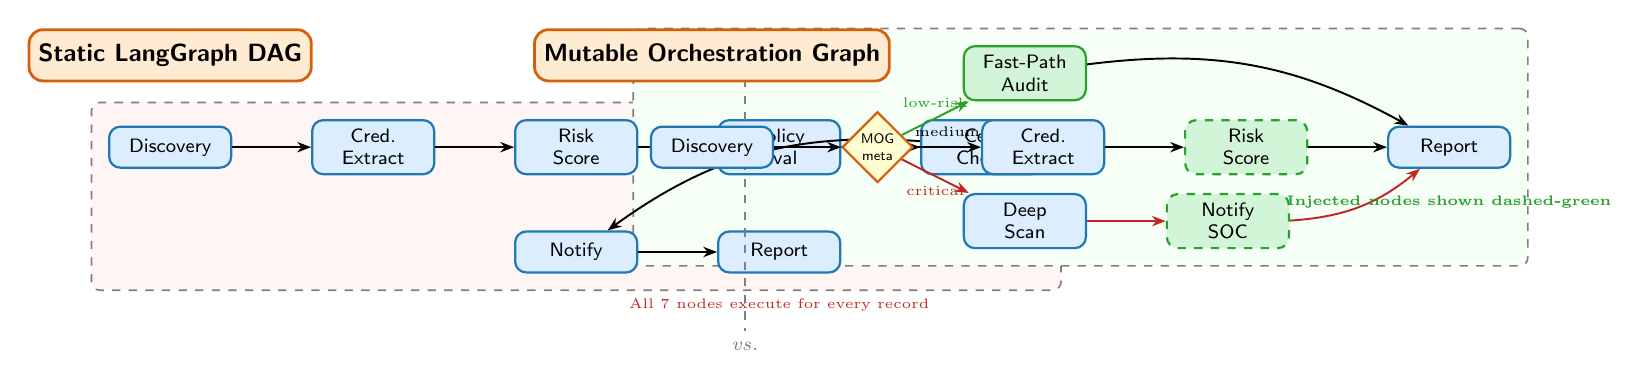
\begin{tikzpicture}[node distance=0.9cm and 1.1cm]

    %% ---- LEFT: Static DAG ----------------------------------------
    \node[meta, minimum width=2.5cm] (sl) {Static LangGraph DAG};

    \node[agent, below=0.55cm of sl] (s1) {Discovery};
    \node[agent, right=1.0cm of s1]  (s2) {Cred.\\ Extract};
    \node[agent, right=1.0cm of s2]  (s3) {Risk\\Score};
    \node[agent, right=1.0cm of s3]  (s4) {Policy\\Eval};
    \node[agent, right=1.0cm of s4]  (s5) {Cert\\Check};
    \node[agent, below=0.7cm of s3]  (s6) {Notify};
    \node[agent, right=1.0cm of s6]  (s7) {Report};

    \draw[arr] (s1)--(s2); \draw[arr] (s2)--(s3);
    \draw[arr] (s3)--(s4); \draw[arr] (s4)--(s5);
    \draw[arr] (s5) to[bend right=20] (s6);
    \draw[arr] (s6)--(s7);

    \node[below=0.2cm of s7, font=\tiny\color{cred}]
      {All 7 nodes execute for every record};

    \begin{scope}[on background layer]
      \node[box, fill=red!4,
            fit=(s1)(s2)(s3)(s4)(s5)(s6)(s7)] {};
    \end{scope}

    %% ---- Divider ---------------------------------------------------
    \draw[dashed, cgray, thick] (7.3,-0.3)--(7.3,-3.5);
    \node[font=\scriptsize\itshape\color{cgray}] at (7.3,-3.7) {vs.};

    %% ---- RIGHT: MOG -----------------------------------------------
    \node[meta, minimum width=2.8cm, right=2.8cm of sl] (ml)
      {Mutable Orchestration Graph};

    \node[agent,  below=0.55cm of ml]        (m1) {Discovery};
    \node[router, right=0.85cm of m1]        (mr) {MOG\\meta};
    \node[agentG, above right=0.35cm and 0.85cm of mr] (m2a)
      {Fast-Path\\Audit};
    \node[agent,  right=0.85cm of mr]        (m2b) {Cred.\\ Extract};
    \node[agent,  below right=0.35cm and 0.85cm of mr] (m2c)
      {Deep\\Scan};
    \node[injected, right=1.0cm of m2b]      (m3)  {Risk\\Score};
    \node[injected, right=1.0cm of m2c]      (m4)  {Notify\\SOC};
    \node[agent,  right=1.0cm of m3]         (m5)  {Report};

    \draw[arr] (m1)--(mr);
    \draw[arr, cgreen] (mr)--(m2a) node[midway,above,font=\tiny]{low-risk};
    \draw[arr] (mr)--(m2b) node[midway,above,font=\tiny]{medium};
    \draw[arr, cred] (mr)--(m2c) node[midway,below,font=\tiny]{critical};
    \draw[arr] (m2a) to[bend left=18] (m5);
    \draw[arr] (m2b)--(m3); \draw[arr] (m3)--(m5);
    \draw[arr, cred] (m2c)--(m4);
    \draw[arr, cred] (m4) to[bend right=18] (m5);

    \node[below=0.22cm of m5, font=\tiny\color{cgreen}]
      {\textbf{Injected nodes shown dashed-green}};

    \begin{scope}[on background layer]
      \node[box, fill=green!4,
            fit=(m1)(mr)(m2a)(m2b)(m2c)(m3)(m4)(m5)] {};
    \end{scope}

  \end{tikzpicture}
  \caption{%
    \textbf{Static DAG vs.\ Mutable Orchestration Graph.}
    Left: the static pipeline executes all seven nodes regardless of
    NHI risk level. Right: the MOG meta-orchestrator routes low-risk
    records through a two-node fast path, medium-risk records through
    the standard path, and critical-risk records through an injected
    \textsc{DeepScan}+\textsc{NotifySOC} subgraph. Dashed-green nodes
    are injected at runtime; no recompilation occurs.}
  \label{fig:lifecycle}
\end{figure*}

%% ------------------------------------------------------------------
%% Figure 2 - System Architecture (double-column)
%% ------------------------------------------------------------------
\begin{figure*}[t]
  \centering
  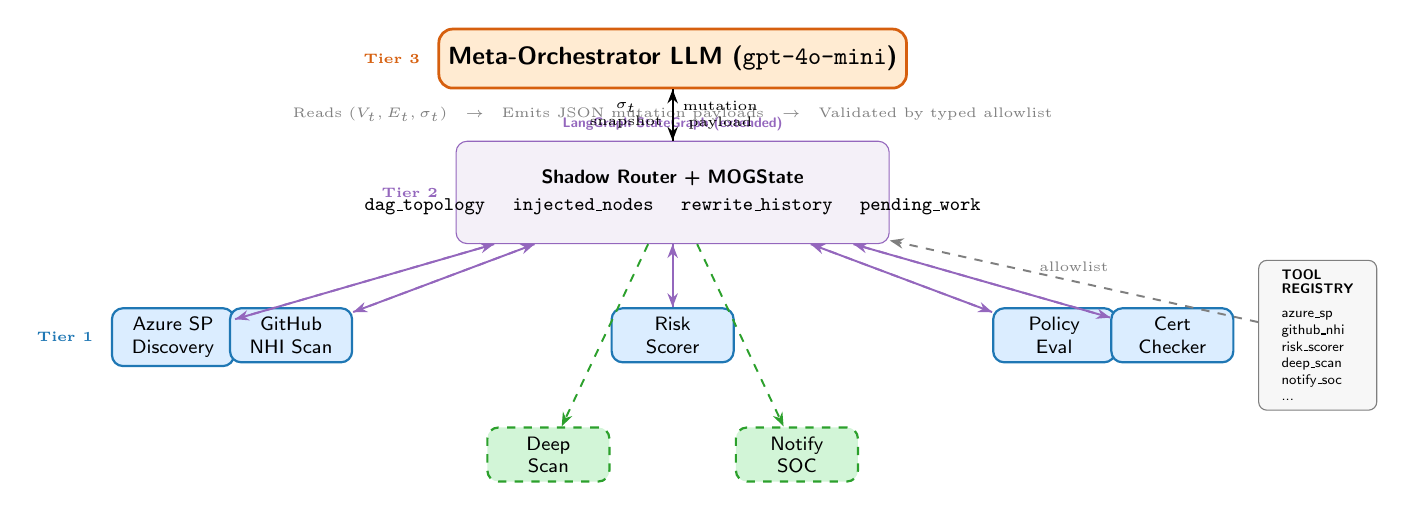
\begin{tikzpicture}[node distance=0.85cm and 1.2cm]

    %% ---- Tier 3: Meta-orchestrator ---------------------------------
    \node[meta, minimum width=5.5cm, minimum height=0.75cm]
      (mo) {Meta-Orchestrator LLM (\texttt{gpt-4o-mini})};

    \node[below=0.1cm of mo, font=\tiny\color{cgray}, align=center]
      {Reads $(V_t,E_t,\sigma_t)$ $\;\;\to\;\;$
       Emits JSON mutation payloads $\;\;\to\;\;$
       Validated by typed allowlist};

    %% ---- Tier 2: Shadow Router + State -----------------------------
    \node[draw=cpurple, fill=cpurple!10, rounded corners=4pt,
          minimum width=5.5cm, minimum height=1.3cm,
          below=0.65cm of mo] (router) {};

    \node[font=\scriptsize\sffamily, at=(router.center), align=center]
      {\textbf{Shadow Router + MOGState} \\[2pt]
       \texttt{dag\_topology} \quad
       \texttt{injected\_nodes} \quad
       \texttt{rewrite\_history} \quad
       \texttt{pending\_work}};
    \node[font=\tiny\color{cpurple}, above=0pt of router.north]
      {\sffamily\bfseries LangGraph StateGraph (extended)};

    %% ---- Tier 1: Worker Agents ------------------------------------
    \node[agent, below left=0.8cm and 2.8cm of router]  (a1) {Azure SP\\Discovery};
    \node[agent, below left=0.8cm and 1.3cm of router]  (a2) {GitHub\\NHI Scan};
    \node[agent, below=0.8cm of router]                 (a3) {Risk\\Scorer};
    \node[agent, below right=0.8cm and 1.3cm of router] (a4) {Policy\\Eval};
    \node[agent, below right=0.8cm and 2.8cm of router] (a5) {Cert\\Checker};
    \node[injected, below left=0.8cm and 0.0cm of a3]   (a6) {Deep\\Scan};
    \node[injected, below right=0.8cm and 0.0cm of a3]  (a7) {Notify\\SOC};

    \foreach \n in {a1,a2,a3,a4,a5}{
      \draw[arr=cpurple] (router)--(\n);
      \draw[arr=cpurple, dashed] (\n)--(router);
    }
    \draw[arr=cgreen, dashed] (router)--(a6);
    \draw[arr=cgreen, dashed] (router)--(a7);

    \draw[arr] (mo)--(router)
      node[midway, right, font=\tiny, align=center] {mutation\\ payload};
    \draw[arr, dashed] (router)--(mo)
      node[midway, left, font=\tiny, align=center] {$\sigma_t$\\ snapshot};

    %% ---- TOOL_REGISTRY label --------------------------------------
    \node[draw=cgray, rounded corners=3pt, fill=gray!6,
          right=0.3cm of a5, minimum width=1.5cm, minimum height=1.1cm,
          font=\tiny\sffamily, align=left]
      (reg) {\textbf{TOOL}\\[-1pt]\textbf{REGISTRY}\\[3pt]
             azure\_sp\\github\_nhi\\risk\_scorer\\deep\_scan\\notify\_soc\\...};
    \draw[arr=cgray, dashed] (reg)--(router)
      node[midway, above, font=\tiny\color{cgray}] {allowlist};

    %% ---- Tier labels -----------------------------------------------
    \node[left=0.1cm of mo, font=\tiny\bfseries\color{corange}]
      {Tier 3};
    \node[left=0.1cm of router, font=\tiny\bfseries\color{cpurple}]
      {Tier 2};
    \node[left=0.1cm of a1, font=\tiny\bfseries\color{cblue}]
      {Tier 1};

  \end{tikzpicture}
  \caption{%
    \textbf{MOG System Architecture.}
    Three tiers: (1)~worker agents execute task logic;
    (2)~the shadow router and \texttt{MOGState} mediate all inter-node
    communication and maintain mutable topology; (3)~the meta-orchestrator
    LLM reads state and emits validated mutation payloads.
    Dashed-green nodes (\textsc{DeepScan}, \textsc{NotifySOC}) are
    injected at runtime and sourced exclusively from \texttt{TOOL\_REGISTRY}.}
  \label{fig:arch}
\end{figure*}

%% ------------------------------------------------------------------
%% Figure 3 - NHI Identity Governance Use Case (double-column)
%% ------------------------------------------------------------------
\begin{figure*}[t]
  \centering
  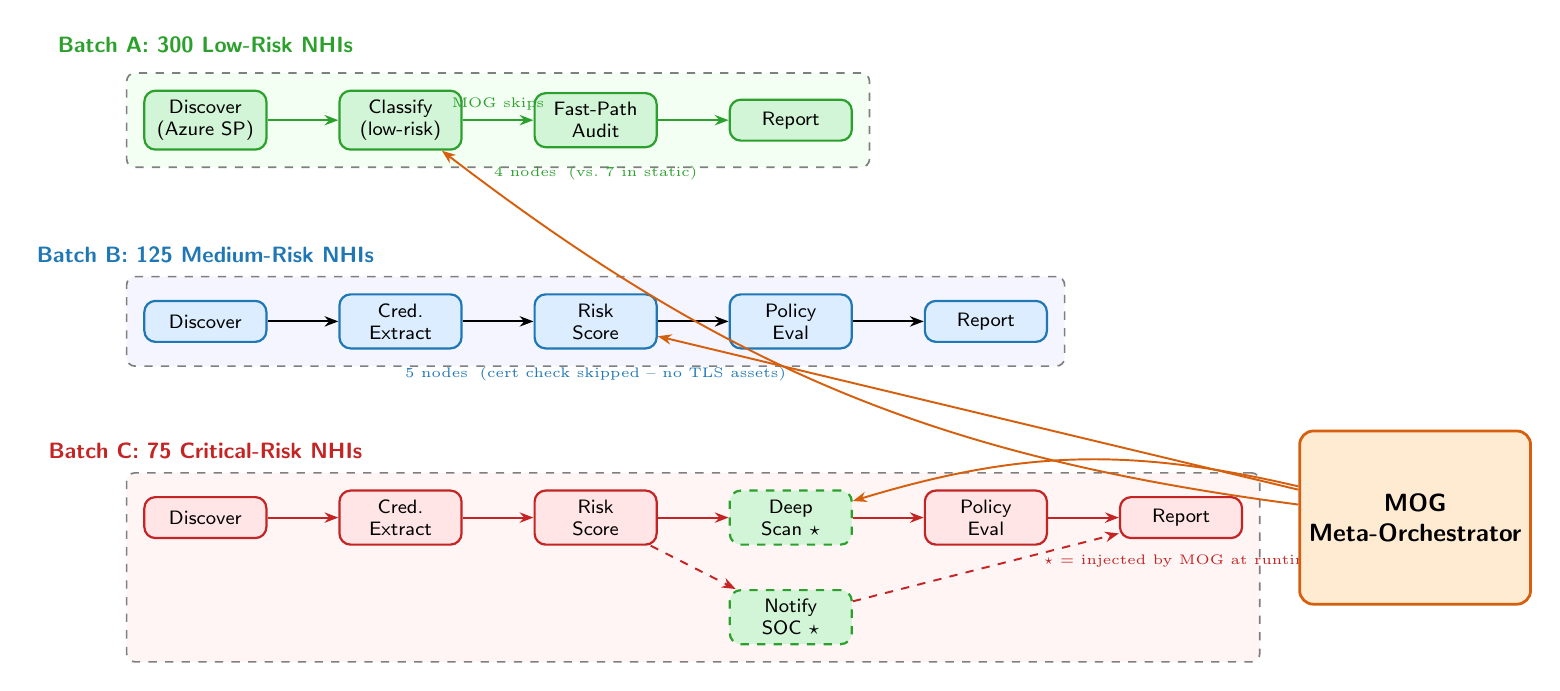
\begin{tikzpicture}[node distance=0.8cm and 0.95cm]

    %% ---- BATCH A: 300 Low-Risk NHIs --------------------------------
    \node[font=\footnotesize\sffamily\bfseries\color{cgreen}]
      (la) {Batch A: 300 Low-Risk NHIs};

    \node[agentG, below=0.35cm of la]  (la1) {Discover\\(Azure SP)};
    \node[agentG, right=0.9cm of la1] (la2) {Classify\\(low-risk)};
    \node[agentG, right=0.9cm of la2] (la3) {Fast-Path\\Audit};
    \node[agentG, right=0.9cm of la3] (la4) {Report};

    \draw[arr=cgreen] (la1)--(la2);
    \draw[arr=cgreen] (la2)--(la3)
      node[midway,above,font=\tiny\color{cgreen}]{MOG skips};
    \draw[arr=cgreen] (la3)--(la4);

    \node[below=0.1cm of la3, font=\tiny\color{cgreen}]
      {4 nodes \;(vs.\ 7 in static)};

    \begin{scope}[on background layer]
      \node[box, fill=green!5,
            fit=(la1)(la2)(la3)(la4)] {};
    \end{scope}

    %% ---- BATCH B: 125 Medium-Risk NHIs ----------------------------
    \node[font=\footnotesize\sffamily\bfseries\color{cblue},
          below=1.1cm of la1] (lb) {Batch B: 125 Medium-Risk NHIs};

    \node[agent, below=0.35cm of lb] (lb1) {Discover};
    \node[agent, right=0.9cm of lb1] (lb2) {Cred.\\Extract};
    \node[agent, right=0.9cm of lb2] (lb3) {Risk\\Score};
    \node[agent, right=0.9cm of lb3] (lb4) {Policy\\Eval};
    \node[agent, right=0.9cm of lb4] (lb5) {Report};

    \draw[arr] (lb1)--(lb2); \draw[arr] (lb2)--(lb3);
    \draw[arr] (lb3)--(lb4); \draw[arr] (lb4)--(lb5);

    \node[below=0.1cm of lb3, font=\tiny\color{cblue}]
      {5 nodes \;(cert check skipped -- no TLS assets)};

    \begin{scope}[on background layer]
      \node[box, fill=blue!4,
            fit=(lb1)(lb2)(lb3)(lb4)(lb5)] {};
    \end{scope}

    %% ---- BATCH C: 75 Critical-Risk NHIs ---------------------------
    \node[font=\footnotesize\sffamily\bfseries\color{cred},
          below=1.15cm of lb1] (lc) {Batch C: 75 Critical-Risk NHIs};

    \node[agentR, below=0.35cm of lc]  (lc1) {Discover};
    \node[agentR, right=0.9cm of lc1]  (lc2) {Cred.\\Extract};
    \node[agentR, right=0.9cm of lc2]  (lc3) {Risk\\Score};
    \node[injected, right=0.9cm of lc3](lc4) {Deep\\Scan $\star$};
    \node[agentR, right=0.9cm of lc4]  (lc5) {Policy\\Eval};
    \node[injected, below=0.55cm of lc4](lc6){Notify\\SOC $\star$};
    \node[agentR, right=0.9cm of lc5]  (lc7) {Report};

    \draw[arr=cred] (lc1)--(lc2); \draw[arr=cred] (lc2)--(lc3);
    \draw[arr=cred] (lc3)--(lc4);
    \draw[arr=cred, dashed] (lc3)--(lc6);
    \draw[arr=cred] (lc4)--(lc5); \draw[arr=cred] (lc5)--(lc7);
    \draw[arr=cred, dashed] (lc6)--(lc7);

    \node[below=0.08cm of lc7, font=\tiny\color{cred}]
      {$\star$ = injected by MOG at runtime};

    \begin{scope}[on background layer]
      \node[box, fill=red!4,
            fit=(lc1)(lc2)(lc3)(lc4)(lc5)(lc6)(lc7)] {};
    \end{scope}

    %% ---- MOG indicator arrow on right ----------------------------
    \node[meta, right=0.7cm of lc7, minimum width=2.1cm,
          minimum height=2.2cm, align=center]
      (mog) {MOG \\ Meta-Orchestrator};

    \draw[arr=corange, bend left=15] (mog) to (la2);
    \draw[arr=corange]               (mog) to (lb3);
    \draw[arr=corange, bend right=15](mog) to (lc4);

  \end{tikzpicture}
  \caption{%
    \textbf{NHI Identity Governance Use Case.}
    The MOG meta-orchestrator routes three concurrent batches through
    structurally distinct subgraphs derived from the same initial DAG.
    Batch~A (low-risk, inactive service principals) skips five nodes.
    Batch~B (medium-risk PATs and deploy keys) follows the standard
    path. Batch~C (critical-risk, expired or over-privileged credentials)
    triggers runtime injection of \textsc{DeepScan} and \textsc{NotifySOC}.
    Dashed-green nodes did not exist at compile time.}
  \label{fig:usecase}
\end{figure*}

%% ------------------------------------------------------------------
%% Figure 4 - Convergence Illustration (single-column)
%% ------------------------------------------------------------------
\begin{figure}[t]
  \centering
  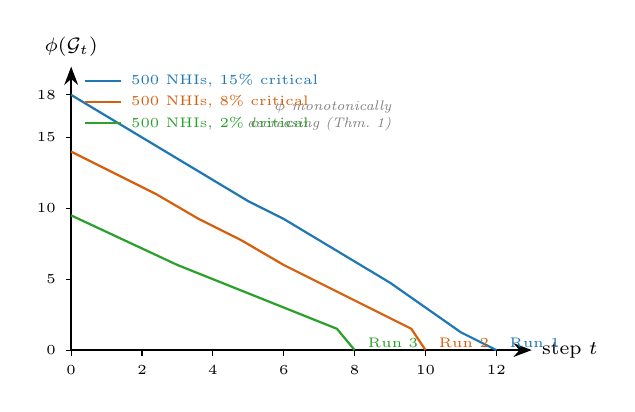
\begin{tikzpicture}[scale=0.9]

    \draw[-{Stealth}, thick] (0,0)--(6.5,0)
      node[right, font=\scriptsize] {step $t$};
    \draw[-{Stealth}, thick] (0,0)--(0,4.0)
      node[above, font=\scriptsize] {$\phi(\mathcal{G}_t)$};

    %% Axis ticks
    \foreach \x/\l in {0/0,1/2,2/4,3/6,4/8,5/10,6/12}{
      \draw (\x,0)--(\x,-0.08)
        node[below,font=\tiny] {\l};
    }
    \foreach \y/\l in {0/0,1/5,2/10,3/15,3.6/18}{
      \draw (0,\y)--(-0.08,\y)
        node[left,font=\tiny] {\l};
    }

    %% Run 1 (blue) - 12 steps
    \draw[cblue, thick]
      (0,3.6)--(0.5,3.3)--(1.0,3.0)--(1.5,2.7)--(2.0,2.4)
      --(2.5,2.1)--(3.0,1.85)--(3.5,1.55)--(4.0,1.25)
      --(4.5,0.95)--(5.0,0.6)--(5.5,0.25)--(6.0,0);
    \node[cblue, right, font=\tiny] at (6.05,0.1) {Run~1};

    %% Run 2 (orange) - 10 steps (fewer critical NHIs)
    \draw[corange, thick]
      (0,2.8)--(0.6,2.5)--(1.2,2.2)--(1.8,1.85)--(2.4,1.55)
      --(3.0,1.2)--(3.6,0.9)--(4.2,0.6)--(4.8,0.3)--(5.0,0);
    \node[corange, right, font=\tiny] at (5.05,0.1) {Run~2};

    %% Run 3 (green) - 8 steps (mostly low-risk)
    \draw[cgreen, thick]
      (0,1.9)--(0.75,1.55)--(1.5,1.2)--(2.25,0.9)
      --(3.0,0.6)--(3.75,0.3)--(4.0,0);
    \node[cgreen, right, font=\tiny] at (4.05,0.1) {Run~3};

    %% Annotation
    \node[font=\tiny\itshape, align=right, text=cgray]
      at (3.5,3.3) {$\phi$ monotonically\\decreasing (Thm.~1)};

    %% Legend
    \draw[cblue, thick] (0.2,3.8)--(0.7,3.8)
      node[right,font=\tiny,cblue] {500 NHIs, 15\% critical};
    \draw[corange, thick] (0.2,3.5)--(0.7,3.5)
      node[right,font=\tiny,corange] {500 NHIs, 8\% critical};
    \draw[cgreen, thick] (0.2,3.2)--(0.7,3.2)
      node[right,font=\tiny,cgreen] {500 NHIs, 2\% critical};

  \end{tikzpicture}
  \caption{%
    \textbf{Convergence of $\phi(\mathcal{G}_t)$ across three runs.}
    Each step corresponds to one worker-node execution followed by
    one meta-orchestrator call. The complexity measure $\phi =
    |V_t| + w(\sigma_t)$ decreases monotonically in all runs,
    confirming Theorem~\ref{thm:term}. Runs with more critical-risk
    NHIs terminate in more steps (injected nodes add to $|V|$) but
    always converge.}
  \label{fig:convergence}
\end{figure}

\end{document}
